% Created by tikzDevice version 0.10.1 on 2020-02-15 16:00:54
% !TEX encoding = UTF-8 Unicode
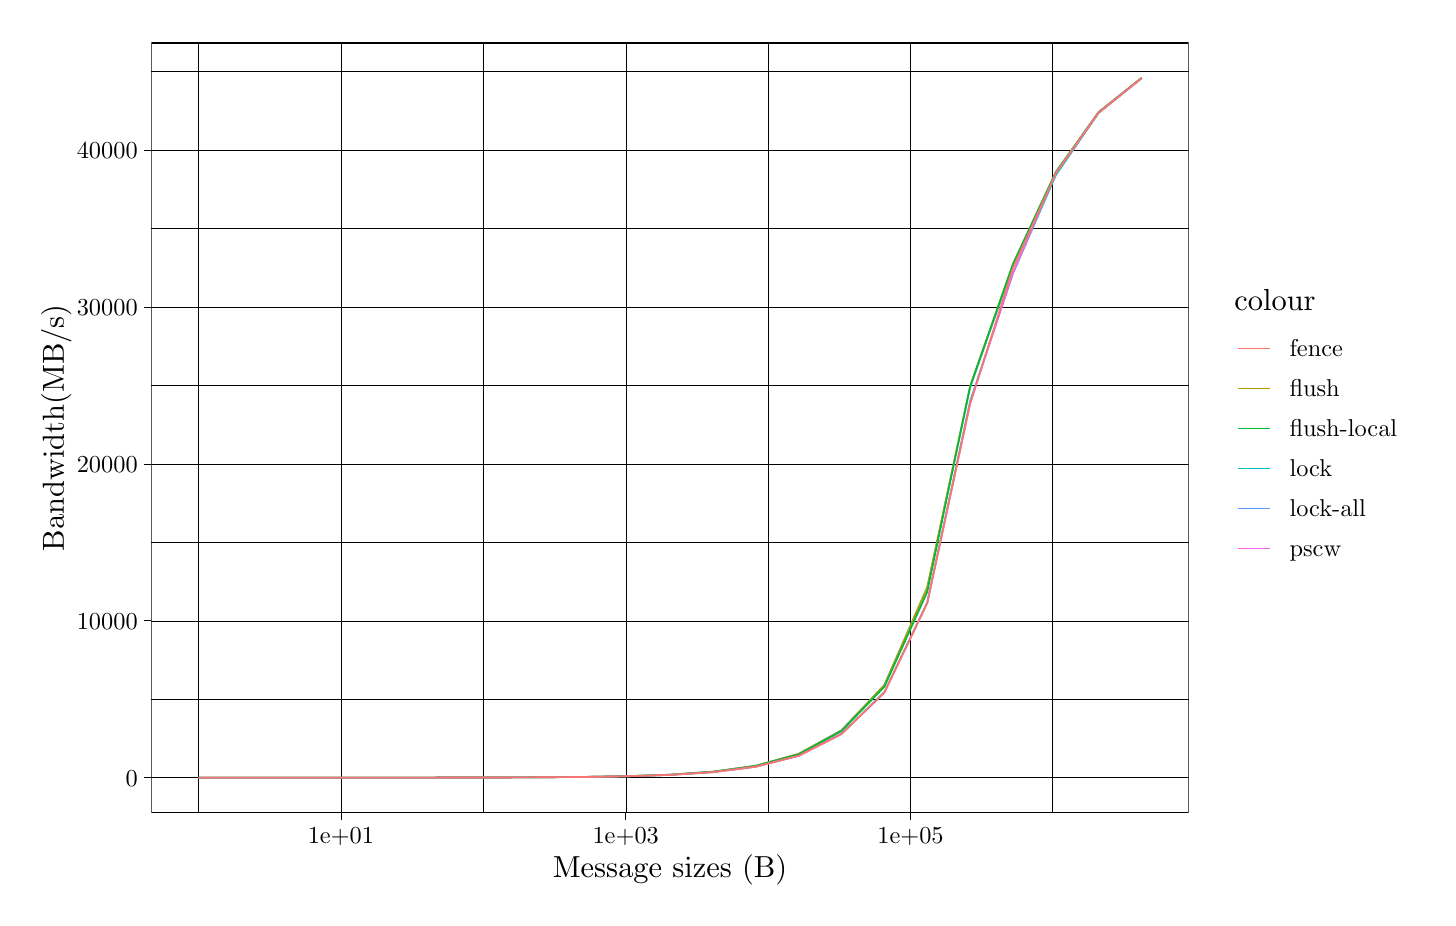
\begin{tikzpicture}[x=1pt,y=1pt]
\definecolor{fillColor}{RGB}{255,255,255}
\path[use as bounding box,fill=fillColor,fill opacity=0.00] (0,0) rectangle (505.89,314.37);
\begin{scope}
\path[clip] (  0.00,  0.00) rectangle (505.89,314.37);
\definecolor{drawColor}{RGB}{255,255,255}
\definecolor{fillColor}{RGB}{255,255,255}

\path[draw=drawColor,line width= 0.6pt,line join=round,line cap=round,fill=fillColor] (  0.00,  0.00) rectangle (505.89,314.37);
\end{scope}
\begin{scope}
\path[clip] ( 44.71, 30.72) rectangle (419.53,308.87);
\definecolor{fillColor}{RGB}{255,255,255}

\path[fill=fillColor] ( 44.71, 30.72) rectangle (419.53,308.87);
\definecolor{drawColor}{RGB}{0,0,0}

\path[draw=drawColor,line width= 0.0pt,line join=round] ( 44.71, 71.70) --
	(419.53, 71.70);

\path[draw=drawColor,line width= 0.0pt,line join=round] ( 44.71,128.36) --
	(419.53,128.36);

\path[draw=drawColor,line width= 0.0pt,line join=round] ( 44.71,185.02) --
	(419.53,185.02);

\path[draw=drawColor,line width= 0.0pt,line join=round] ( 44.71,241.68) --
	(419.53,241.68);

\path[draw=drawColor,line width= 0.0pt,line join=round] ( 44.71,298.35) --
	(419.53,298.35);

\path[draw=drawColor,line width= 0.0pt,line join=round] ( 61.75, 30.72) --
	( 61.75,308.87);

\path[draw=drawColor,line width= 0.0pt,line join=round] (164.65, 30.72) --
	(164.65,308.87);

\path[draw=drawColor,line width= 0.0pt,line join=round] (267.55, 30.72) --
	(267.55,308.87);

\path[draw=drawColor,line width= 0.0pt,line join=round] (370.46, 30.72) --
	(370.46,308.87);

\path[draw=drawColor,line width= 0.1pt,line join=round] ( 44.71, 43.37) --
	(419.53, 43.37);

\path[draw=drawColor,line width= 0.1pt,line join=round] ( 44.71,100.03) --
	(419.53,100.03);

\path[draw=drawColor,line width= 0.1pt,line join=round] ( 44.71,156.69) --
	(419.53,156.69);

\path[draw=drawColor,line width= 0.1pt,line join=round] ( 44.71,213.35) --
	(419.53,213.35);

\path[draw=drawColor,line width= 0.1pt,line join=round] ( 44.71,270.02) --
	(419.53,270.02);

\path[draw=drawColor,line width= 0.1pt,line join=round] (113.20, 30.72) --
	(113.20,308.87);

\path[draw=drawColor,line width= 0.1pt,line join=round] (216.10, 30.72) --
	(216.10,308.87);

\path[draw=drawColor,line width= 0.1pt,line join=round] (319.01, 30.72) --
	(319.01,308.87);
\definecolor{drawColor}{RGB}{97,156,255}

\path[draw=drawColor,line width= 0.6pt,line join=round] ( 61.75, 43.37) --
	( 77.24, 43.37) --
	( 92.73, 43.37) --
	(108.22, 43.37) --
	(123.70, 43.38) --
	(139.19, 43.38) --
	(154.68, 43.40) --
	(170.17, 43.43) --
	(185.66, 43.50) --
	(201.15, 43.64) --
	(216.63, 43.90) --
	(232.12, 44.44) --
	(247.61, 45.52) --
	(263.10, 47.66) --
	(278.59, 51.96) --
	(294.08, 60.52) --
	(309.56, 76.84) --
	(325.05,112.12) --
	(340.54,184.33) --
	(356.03,228.24) --
	(371.52,261.69) --
	(387.00,283.58) --
	(402.49,296.05);
\definecolor{drawColor}{RGB}{0,191,196}

\path[draw=drawColor,line width= 0.6pt,line join=round] ( 61.75, 43.37) --
	( 77.24, 43.37) --
	( 92.73, 43.37) --
	(108.22, 43.37) --
	(123.70, 43.38) --
	(139.19, 43.38) --
	(154.68, 43.40) --
	(170.17, 43.43) --
	(185.66, 43.49) --
	(201.15, 43.62) --
	(216.63, 43.86) --
	(232.12, 44.36) --
	(247.61, 45.36) --
	(263.10, 47.33) --
	(278.59, 51.31) --
	(294.08, 59.27) --
	(309.56, 74.29) --
	(325.05,106.62) --
	(340.54,179.36) --
	(356.03,225.59) --
	(371.52,261.07) --
	(387.00,283.63) --
	(402.49,296.09);
\definecolor{drawColor}{RGB}{183,159,0}

\path[draw=drawColor,line width= 0.6pt,line join=round] ( 61.75, 43.37) --
	( 77.24, 43.37) --
	( 92.73, 43.37) --
	(108.22, 43.37) --
	(123.70, 43.38) --
	(139.19, 43.38) --
	(154.68, 43.40) --
	(170.17, 43.43) --
	(185.66, 43.50) --
	(201.15, 43.64) --
	(216.63, 43.91) --
	(232.12, 44.44) --
	(247.61, 45.52) --
	(263.10, 47.67) --
	(278.59, 51.95) --
	(294.08, 60.43) --
	(309.56, 76.82) --
	(325.05,112.08) --
	(340.54,184.87) --
	(356.03,228.92) --
	(371.52,262.20) --
	(387.00,283.89) --
	(402.49,296.23);
\definecolor{drawColor}{RGB}{0,186,56}

\path[draw=drawColor,line width= 0.6pt,line join=round] ( 61.75, 43.37) --
	( 77.24, 43.37) --
	( 92.73, 43.37) --
	(108.22, 43.37) --
	(123.70, 43.38) --
	(139.19, 43.38) --
	(154.68, 43.40) --
	(170.17, 43.43) --
	(185.66, 43.50) --
	(201.15, 43.63) --
	(216.63, 43.89) --
	(232.12, 44.42) --
	(247.61, 45.49) --
	(263.10, 47.59) --
	(278.59, 51.77) --
	(294.08, 60.20) --
	(309.56, 76.19) --
	(325.05,110.43) --
	(340.54,184.61) --
	(356.03,228.96) --
	(371.52,262.18) --
	(387.00,283.87) --
	(402.49,296.22);
\definecolor{drawColor}{RGB}{245,100,227}

\path[draw=drawColor,line width= 0.6pt,line join=round] ( 61.75, 43.37) --
	( 77.24, 43.37) --
	( 92.73, 43.37) --
	(108.22, 43.37) --
	(123.70, 43.38) --
	(139.19, 43.38) --
	(154.68, 43.40) --
	(170.17, 43.43) --
	(185.66, 43.49) --
	(201.15, 43.62) --
	(216.63, 43.86) --
	(232.12, 44.36) --
	(247.61, 45.35) --
	(263.10, 47.32) --
	(278.59, 51.27) --
	(294.08, 59.23) --
	(309.56, 74.08) --
	(325.05,106.51) --
	(340.54,178.77) --
	(356.03,225.70) --
	(371.52,261.82) --
	(387.00,283.74) --
	(402.49,296.13);
\definecolor{drawColor}{RGB}{248,118,109}

\path[draw=drawColor,line width= 0.6pt,line join=round] ( 61.75, 43.37) --
	( 77.24, 43.37) --
	( 92.73, 43.37) --
	(108.22, 43.37) --
	(123.70, 43.38) --
	(139.19, 43.38) --
	(154.68, 43.40) --
	(170.17, 43.43) --
	(185.66, 43.49) --
	(201.15, 43.61) --
	(216.63, 43.86) --
	(232.12, 44.35) --
	(247.61, 45.34) --
	(263.10, 47.31) --
	(278.59, 51.25) --
	(294.08, 59.08) --
	(309.56, 74.12) --
	(325.05,106.39) --
	(340.54,178.29) --
	(356.03,227.55) --
	(371.52,261.74) --
	(387.00,283.62) --
	(402.49,296.08);
\definecolor{drawColor}{RGB}{0,0,0}

\path[draw=drawColor,line width= 0.6pt,line join=round,line cap=round] ( 44.71, 30.72) rectangle (419.53,308.87);
\end{scope}
\begin{scope}
\path[clip] (  0.00,  0.00) rectangle (505.89,314.37);
\definecolor{drawColor}{RGB}{0,0,0}

\node[text=drawColor,anchor=base east,inner sep=0pt, outer sep=0pt, scale=  0.88] at ( 39.76, 40.34) {0};

\node[text=drawColor,anchor=base east,inner sep=0pt, outer sep=0pt, scale=  0.88] at ( 39.76, 97.00) {10000};

\node[text=drawColor,anchor=base east,inner sep=0pt, outer sep=0pt, scale=  0.88] at ( 39.76,153.66) {20000};

\node[text=drawColor,anchor=base east,inner sep=0pt, outer sep=0pt, scale=  0.88] at ( 39.76,210.32) {30000};

\node[text=drawColor,anchor=base east,inner sep=0pt, outer sep=0pt, scale=  0.88] at ( 39.76,266.99) {40000};
\end{scope}
\begin{scope}
\path[clip] (  0.00,  0.00) rectangle (505.89,314.37);
\definecolor{drawColor}{RGB}{0,0,0}

\path[draw=drawColor,line width= 0.3pt,line join=round] ( 41.96, 43.37) --
	( 44.71, 43.37);

\path[draw=drawColor,line width= 0.3pt,line join=round] ( 41.96,100.03) --
	( 44.71,100.03);

\path[draw=drawColor,line width= 0.3pt,line join=round] ( 41.96,156.69) --
	( 44.71,156.69);

\path[draw=drawColor,line width= 0.3pt,line join=round] ( 41.96,213.35) --
	( 44.71,213.35);

\path[draw=drawColor,line width= 0.3pt,line join=round] ( 41.96,270.02) --
	( 44.71,270.02);
\end{scope}
\begin{scope}
\path[clip] (  0.00,  0.00) rectangle (505.89,314.37);
\definecolor{drawColor}{RGB}{0,0,0}

\path[draw=drawColor,line width= 0.3pt,line join=round] (113.20, 27.97) --
	(113.20, 30.72);

\path[draw=drawColor,line width= 0.3pt,line join=round] (216.10, 27.97) --
	(216.10, 30.72);

\path[draw=drawColor,line width= 0.3pt,line join=round] (319.01, 27.97) --
	(319.01, 30.72);
\end{scope}
\begin{scope}
\path[clip] (  0.00,  0.00) rectangle (505.89,314.37);
\definecolor{drawColor}{RGB}{0,0,0}

\node[text=drawColor,anchor=base,inner sep=0pt, outer sep=0pt, scale=  0.88] at (113.20, 19.71) {1e+01};

\node[text=drawColor,anchor=base,inner sep=0pt, outer sep=0pt, scale=  0.88] at (216.10, 19.71) {1e+03};

\node[text=drawColor,anchor=base,inner sep=0pt, outer sep=0pt, scale=  0.88] at (319.01, 19.71) {1e+05};
\end{scope}
\begin{scope}
\path[clip] (  0.00,  0.00) rectangle (505.89,314.37);
\definecolor{drawColor}{RGB}{0,0,0}

\node[text=drawColor,anchor=base,inner sep=0pt, outer sep=0pt, scale=  1.10] at (232.12,  7.44) {Message sizes (B)};
\end{scope}
\begin{scope}
\path[clip] (  0.00,  0.00) rectangle (505.89,314.37);
\definecolor{drawColor}{RGB}{0,0,0}

\node[text=drawColor,rotate= 90.00,anchor=base,inner sep=0pt, outer sep=0pt, scale=  1.10] at ( 13.08,169.80) {Bandwidth(MB/s)};
\end{scope}
\begin{scope}
\path[clip] (  0.00,  0.00) rectangle (505.89,314.37);
\definecolor{fillColor}{RGB}{255,255,255}

\path[fill=fillColor] (430.53,113.43) rectangle (500.39,226.17);
\end{scope}
\begin{scope}
\path[clip] (  0.00,  0.00) rectangle (505.89,314.37);
\definecolor{drawColor}{RGB}{0,0,0}

\node[text=drawColor,anchor=base west,inner sep=0pt, outer sep=0pt, scale=  1.10] at (436.03,212.12) {colour};
\end{scope}
\begin{scope}
\path[clip] (  0.00,  0.00) rectangle (505.89,314.37);
\definecolor{fillColor}{RGB}{255,255,255}

\path[fill=fillColor] (436.03,191.20) rectangle (450.48,205.65);
\end{scope}
\begin{scope}
\path[clip] (  0.00,  0.00) rectangle (505.89,314.37);
\definecolor{drawColor}{RGB}{248,118,109}

\path[draw=drawColor,line width= 0.6pt,line join=round] (437.48,198.42) -- (449.04,198.42);
\end{scope}
\begin{scope}
\path[clip] (  0.00,  0.00) rectangle (505.89,314.37);
\definecolor{drawColor}{RGB}{248,118,109}

\path[draw=drawColor,line width= 0.6pt,line join=round] (437.48,198.42) -- (449.04,198.42);
\end{scope}
\begin{scope}
\path[clip] (  0.00,  0.00) rectangle (505.89,314.37);
\definecolor{drawColor}{RGB}{248,118,109}

\path[draw=drawColor,line width= 0.6pt,line join=round] (437.48,198.42) -- (449.04,198.42);
\end{scope}
\begin{scope}
\path[clip] (  0.00,  0.00) rectangle (505.89,314.37);
\definecolor{drawColor}{RGB}{248,118,109}

\path[draw=drawColor,line width= 0.6pt,line join=round] (437.48,198.42) -- (449.04,198.42);
\end{scope}
\begin{scope}
\path[clip] (  0.00,  0.00) rectangle (505.89,314.37);
\definecolor{drawColor}{RGB}{248,118,109}

\path[draw=drawColor,line width= 0.6pt,line join=round] (437.48,198.42) -- (449.04,198.42);
\end{scope}
\begin{scope}
\path[clip] (  0.00,  0.00) rectangle (505.89,314.37);
\definecolor{drawColor}{RGB}{248,118,109}

\path[draw=drawColor,line width= 0.6pt,line join=round] (437.48,198.42) -- (449.04,198.42);
\end{scope}
\begin{scope}
\path[clip] (  0.00,  0.00) rectangle (505.89,314.37);
\definecolor{fillColor}{RGB}{255,255,255}

\path[fill=fillColor] (436.03,176.74) rectangle (450.48,191.20);
\end{scope}
\begin{scope}
\path[clip] (  0.00,  0.00) rectangle (505.89,314.37);
\definecolor{drawColor}{RGB}{183,159,0}

\path[draw=drawColor,line width= 0.6pt,line join=round] (437.48,183.97) -- (449.04,183.97);
\end{scope}
\begin{scope}
\path[clip] (  0.00,  0.00) rectangle (505.89,314.37);
\definecolor{drawColor}{RGB}{183,159,0}

\path[draw=drawColor,line width= 0.6pt,line join=round] (437.48,183.97) -- (449.04,183.97);
\end{scope}
\begin{scope}
\path[clip] (  0.00,  0.00) rectangle (505.89,314.37);
\definecolor{drawColor}{RGB}{183,159,0}

\path[draw=drawColor,line width= 0.6pt,line join=round] (437.48,183.97) -- (449.04,183.97);
\end{scope}
\begin{scope}
\path[clip] (  0.00,  0.00) rectangle (505.89,314.37);
\definecolor{drawColor}{RGB}{183,159,0}

\path[draw=drawColor,line width= 0.6pt,line join=round] (437.48,183.97) -- (449.04,183.97);
\end{scope}
\begin{scope}
\path[clip] (  0.00,  0.00) rectangle (505.89,314.37);
\definecolor{drawColor}{RGB}{183,159,0}

\path[draw=drawColor,line width= 0.6pt,line join=round] (437.48,183.97) -- (449.04,183.97);
\end{scope}
\begin{scope}
\path[clip] (  0.00,  0.00) rectangle (505.89,314.37);
\definecolor{drawColor}{RGB}{183,159,0}

\path[draw=drawColor,line width= 0.6pt,line join=round] (437.48,183.97) -- (449.04,183.97);
\end{scope}
\begin{scope}
\path[clip] (  0.00,  0.00) rectangle (505.89,314.37);
\definecolor{fillColor}{RGB}{255,255,255}

\path[fill=fillColor] (436.03,162.29) rectangle (450.48,176.74);
\end{scope}
\begin{scope}
\path[clip] (  0.00,  0.00) rectangle (505.89,314.37);
\definecolor{drawColor}{RGB}{0,186,56}

\path[draw=drawColor,line width= 0.6pt,line join=round] (437.48,169.52) -- (449.04,169.52);
\end{scope}
\begin{scope}
\path[clip] (  0.00,  0.00) rectangle (505.89,314.37);
\definecolor{drawColor}{RGB}{0,186,56}

\path[draw=drawColor,line width= 0.6pt,line join=round] (437.48,169.52) -- (449.04,169.52);
\end{scope}
\begin{scope}
\path[clip] (  0.00,  0.00) rectangle (505.89,314.37);
\definecolor{drawColor}{RGB}{0,186,56}

\path[draw=drawColor,line width= 0.6pt,line join=round] (437.48,169.52) -- (449.04,169.52);
\end{scope}
\begin{scope}
\path[clip] (  0.00,  0.00) rectangle (505.89,314.37);
\definecolor{drawColor}{RGB}{0,186,56}

\path[draw=drawColor,line width= 0.6pt,line join=round] (437.48,169.52) -- (449.04,169.52);
\end{scope}
\begin{scope}
\path[clip] (  0.00,  0.00) rectangle (505.89,314.37);
\definecolor{drawColor}{RGB}{0,186,56}

\path[draw=drawColor,line width= 0.6pt,line join=round] (437.48,169.52) -- (449.04,169.52);
\end{scope}
\begin{scope}
\path[clip] (  0.00,  0.00) rectangle (505.89,314.37);
\definecolor{drawColor}{RGB}{0,186,56}

\path[draw=drawColor,line width= 0.6pt,line join=round] (437.48,169.52) -- (449.04,169.52);
\end{scope}
\begin{scope}
\path[clip] (  0.00,  0.00) rectangle (505.89,314.37);
\definecolor{fillColor}{RGB}{255,255,255}

\path[fill=fillColor] (436.03,147.84) rectangle (450.48,162.29);
\end{scope}
\begin{scope}
\path[clip] (  0.00,  0.00) rectangle (505.89,314.37);
\definecolor{drawColor}{RGB}{0,191,196}

\path[draw=drawColor,line width= 0.6pt,line join=round] (437.48,155.06) -- (449.04,155.06);
\end{scope}
\begin{scope}
\path[clip] (  0.00,  0.00) rectangle (505.89,314.37);
\definecolor{drawColor}{RGB}{0,191,196}

\path[draw=drawColor,line width= 0.6pt,line join=round] (437.48,155.06) -- (449.04,155.06);
\end{scope}
\begin{scope}
\path[clip] (  0.00,  0.00) rectangle (505.89,314.37);
\definecolor{drawColor}{RGB}{0,191,196}

\path[draw=drawColor,line width= 0.6pt,line join=round] (437.48,155.06) -- (449.04,155.06);
\end{scope}
\begin{scope}
\path[clip] (  0.00,  0.00) rectangle (505.89,314.37);
\definecolor{drawColor}{RGB}{0,191,196}

\path[draw=drawColor,line width= 0.6pt,line join=round] (437.48,155.06) -- (449.04,155.06);
\end{scope}
\begin{scope}
\path[clip] (  0.00,  0.00) rectangle (505.89,314.37);
\definecolor{drawColor}{RGB}{0,191,196}

\path[draw=drawColor,line width= 0.6pt,line join=round] (437.48,155.06) -- (449.04,155.06);
\end{scope}
\begin{scope}
\path[clip] (  0.00,  0.00) rectangle (505.89,314.37);
\definecolor{drawColor}{RGB}{0,191,196}

\path[draw=drawColor,line width= 0.6pt,line join=round] (437.48,155.06) -- (449.04,155.06);
\end{scope}
\begin{scope}
\path[clip] (  0.00,  0.00) rectangle (505.89,314.37);
\definecolor{fillColor}{RGB}{255,255,255}

\path[fill=fillColor] (436.03,133.38) rectangle (450.48,147.84);
\end{scope}
\begin{scope}
\path[clip] (  0.00,  0.00) rectangle (505.89,314.37);
\definecolor{drawColor}{RGB}{97,156,255}

\path[draw=drawColor,line width= 0.6pt,line join=round] (437.48,140.61) -- (449.04,140.61);
\end{scope}
\begin{scope}
\path[clip] (  0.00,  0.00) rectangle (505.89,314.37);
\definecolor{drawColor}{RGB}{97,156,255}

\path[draw=drawColor,line width= 0.6pt,line join=round] (437.48,140.61) -- (449.04,140.61);
\end{scope}
\begin{scope}
\path[clip] (  0.00,  0.00) rectangle (505.89,314.37);
\definecolor{drawColor}{RGB}{97,156,255}

\path[draw=drawColor,line width= 0.6pt,line join=round] (437.48,140.61) -- (449.04,140.61);
\end{scope}
\begin{scope}
\path[clip] (  0.00,  0.00) rectangle (505.89,314.37);
\definecolor{drawColor}{RGB}{97,156,255}

\path[draw=drawColor,line width= 0.6pt,line join=round] (437.48,140.61) -- (449.04,140.61);
\end{scope}
\begin{scope}
\path[clip] (  0.00,  0.00) rectangle (505.89,314.37);
\definecolor{drawColor}{RGB}{97,156,255}

\path[draw=drawColor,line width= 0.6pt,line join=round] (437.48,140.61) -- (449.04,140.61);
\end{scope}
\begin{scope}
\path[clip] (  0.00,  0.00) rectangle (505.89,314.37);
\definecolor{drawColor}{RGB}{97,156,255}

\path[draw=drawColor,line width= 0.6pt,line join=round] (437.48,140.61) -- (449.04,140.61);
\end{scope}
\begin{scope}
\path[clip] (  0.00,  0.00) rectangle (505.89,314.37);
\definecolor{fillColor}{RGB}{255,255,255}

\path[fill=fillColor] (436.03,118.93) rectangle (450.48,133.38);
\end{scope}
\begin{scope}
\path[clip] (  0.00,  0.00) rectangle (505.89,314.37);
\definecolor{drawColor}{RGB}{245,100,227}

\path[draw=drawColor,line width= 0.6pt,line join=round] (437.48,126.15) -- (449.04,126.15);
\end{scope}
\begin{scope}
\path[clip] (  0.00,  0.00) rectangle (505.89,314.37);
\definecolor{drawColor}{RGB}{245,100,227}

\path[draw=drawColor,line width= 0.6pt,line join=round] (437.48,126.15) -- (449.04,126.15);
\end{scope}
\begin{scope}
\path[clip] (  0.00,  0.00) rectangle (505.89,314.37);
\definecolor{drawColor}{RGB}{245,100,227}

\path[draw=drawColor,line width= 0.6pt,line join=round] (437.48,126.15) -- (449.04,126.15);
\end{scope}
\begin{scope}
\path[clip] (  0.00,  0.00) rectangle (505.89,314.37);
\definecolor{drawColor}{RGB}{245,100,227}

\path[draw=drawColor,line width= 0.6pt,line join=round] (437.48,126.15) -- (449.04,126.15);
\end{scope}
\begin{scope}
\path[clip] (  0.00,  0.00) rectangle (505.89,314.37);
\definecolor{drawColor}{RGB}{245,100,227}

\path[draw=drawColor,line width= 0.6pt,line join=round] (437.48,126.15) -- (449.04,126.15);
\end{scope}
\begin{scope}
\path[clip] (  0.00,  0.00) rectangle (505.89,314.37);
\definecolor{drawColor}{RGB}{245,100,227}

\path[draw=drawColor,line width= 0.6pt,line join=round] (437.48,126.15) -- (449.04,126.15);
\end{scope}
\begin{scope}
\path[clip] (  0.00,  0.00) rectangle (505.89,314.37);
\definecolor{drawColor}{RGB}{0,0,0}

\node[text=drawColor,anchor=base west,inner sep=0pt, outer sep=0pt, scale=  0.88] at (455.98,195.39) {fence};
\end{scope}
\begin{scope}
\path[clip] (  0.00,  0.00) rectangle (505.89,314.37);
\definecolor{drawColor}{RGB}{0,0,0}

\node[text=drawColor,anchor=base west,inner sep=0pt, outer sep=0pt, scale=  0.88] at (455.98,180.94) {flush};
\end{scope}
\begin{scope}
\path[clip] (  0.00,  0.00) rectangle (505.89,314.37);
\definecolor{drawColor}{RGB}{0,0,0}

\node[text=drawColor,anchor=base west,inner sep=0pt, outer sep=0pt, scale=  0.88] at (455.98,166.49) {flush-local};
\end{scope}
\begin{scope}
\path[clip] (  0.00,  0.00) rectangle (505.89,314.37);
\definecolor{drawColor}{RGB}{0,0,0}

\node[text=drawColor,anchor=base west,inner sep=0pt, outer sep=0pt, scale=  0.88] at (455.98,152.03) {lock};
\end{scope}
\begin{scope}
\path[clip] (  0.00,  0.00) rectangle (505.89,314.37);
\definecolor{drawColor}{RGB}{0,0,0}

\node[text=drawColor,anchor=base west,inner sep=0pt, outer sep=0pt, scale=  0.88] at (455.98,137.58) {lock-all};
\end{scope}
\begin{scope}
\path[clip] (  0.00,  0.00) rectangle (505.89,314.37);
\definecolor{drawColor}{RGB}{0,0,0}

\node[text=drawColor,anchor=base west,inner sep=0pt, outer sep=0pt, scale=  0.88] at (455.98,123.12) {pscw};
\end{scope}
\end{tikzpicture}
